\documentclass{beamer}
\usetheme{Madrid}

% pdflatex
\usepackage[utf8]{inputenc}
\usepackage[T2A]{fontenc}
\usepackage[russian,english]{babel}
\usepackage{cmap}
\usepackage{babel}

\usepackage{graphicx}
\usepackage{xcolor}
\usepackage{tikz}
\usepackage{amsmath,amssymb,amsthm}
\usepackage{mathtools}
\usepackage{listings}
\usepackage{booktabs}
\usepackage{array}
\usetikzlibrary{arrows.meta,positioning,shapes.geometric,fit,backgrounds,calc,decorations.pathreplacing}

% Footline: show current section (left) and frame numbers (right)
\setbeamertemplate{footline}{%
  \leavevmode%
  \hbox{%
    \begin{beamercolorbox}[wd=.78\paperwidth,ht=2.5ex,dp=1ex,left]{author in head/foot}%
      \hspace*{1em}\usebeamerfont{footline}\insertsectionhead%
    \end{beamercolorbox}%
    \begin{beamercolorbox}[wd=.22\paperwidth,ht=2.5ex,dp=1ex,right]{date in head/foot}%
      \usebeamerfont{footline}\insertframenumber{} / \inserttotalframenumber\hspace*{1em}%
    \end{beamercolorbox}%
  }%
}

\newcommand{\parpause}[1]{\only<+->{#1\par}}
\newenvironment{definitionbox}[1][Определение]{%
  \begin{exampleblock}{#1}
}{%
  \end{exampleblock}
}

\AtBeginSection[]
{
  \begin{frame}
    \frametitle{Содержание}
    \tableofcontents[currentsection]
  \end{frame}
}

\title{Семинар 11. Распределенные файловые системы: NFS, GFS, HDFS, IPFS}
\subtitle{Распределенные вычисления}
\author{Георгий Семенов}
\institute{Институт прикладных компьютерных наук \\ Университет ИТМО}
\date{весна 2026}

\begin{document}

\frame{\titlepage}

\begin{frame}
\frametitle{Организационные моменты}

\begin{itemize}
  \item Через неделю – (7 мая, 23:59) дедлайн по домашнему заданию 
\end{itemize}

\end{frame}

\section{<<Обычные>> файловые системы: FAT, NTFS, ext4}

\begin{frame}
\frametitle{Понятие файловой системы}

\begin{definitionbox}[Файловая система]
  Это программное обеспечение, которое управляет тем, как данные хранятся и извлекаются на запоминающем устройстве.
\end{definitionbox}

\textbf{Основные задачи:}
\begin{itemize}
  \item Организация данных в файлы и каталоги
  \item Управление пространством на диске
  \item Контроль доступа к файлам (права доступа)
  \item Отслеживание метаданных (имя, размер, время создания)
  \item Обеспечение надежности данных
\end{itemize}

\end{frame}

\begin{frame}
\frametitle{FAT (File Allocation Table)}

\textbf{История:} разработана компанией Microsoft в 1977 году для дискет, позже использовалась для жёстких дисков

\textbf{Структура:}
\begin{itemize}
  \item \textbf{Boot sector} — загрузочный сектор с информацией о ФС
  \item \textbf{File Allocation Table} — таблица распределения (несколько копий)
  \item \textbf{Root directory} — корневой каталог
  \item \textbf{Data area} — область данных
\end{itemize}

\textbf{Варианты:} FAT12 (дискеты), FAT16, FAT32

\textbf{Недостатки:}
\begin{itemize}
  \item Нет встроенной защиты доступа
  \item Фрагментация диска
  \item Ограничения на размер файлов (FAT32: 4 GB)
\end{itemize}

\end{frame}

\begin{frame}
\frametitle{Структура таблицы}

\begin{center}
    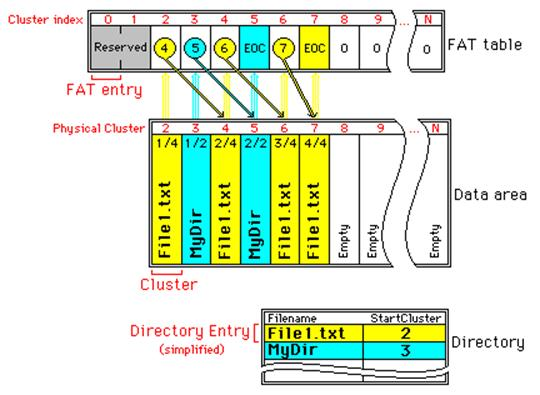
\includegraphics[width=0.8\linewidth,keepaspectratio]{images/fat12.jpg}
\end{center}

\href{https://students.cs.byu.edu/~cs345ta/labs/P6-FAT\%20Supplement.html}{Подробнее про FAT}

\end{frame}

\begin{frame}
\frametitle{NTFS (NT File System)}

\textbf{История:} разработана Microsoft для Windows NT (1993), стандарт для Windows

\textbf{Ключевые возможности:}
\begin{itemize}
  \item Журналирование (journaling) для надежности
  \item Файлы больше 4 GB и диски больше 2 TB
  \item Контроль доступа (ACL — Access Control Lists)
  \item Шифрование файлов (EFS)
  \item Жесткие и символические ссылки
\end{itemize}

\textbf{Структура:}
\begin{itemize}
  \item \textbf{MFT} (Master File Table) — основная таблица файлов
  \item Каждый файл — это набор атрибутов в MFT
\end{itemize}

\textbf{Сравнение с FAT:} FAT проще, но NTFS надежнее и функциональнее

\end{frame}

\begin{frame}
\frametitle{Структура таблицы}

\begin{center}
    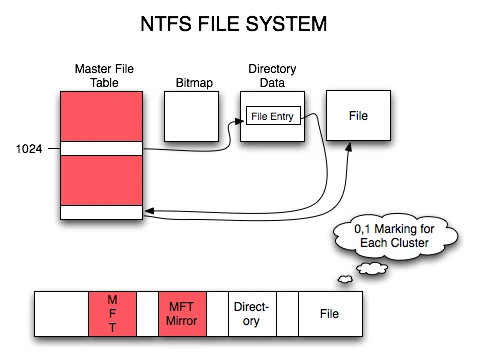
\includegraphics[width=0.8\linewidth,keepaspectratio]{images/ntfs-file-system.png}
\end{center}

\end{frame}

\begin{frame}
\frametitle{Файловые системы в Linux: ext4}

\textbf{История линейки ext:} ext (1992) → ext2 (1993) → ext3 (2001) → ext4 (2008)

\textbf{ext4 особенности:}
\begin{itemize}
  \item Журналирование (как NTFS)
  \item Extents вместо блок-карт (улучшена фрагментация)
  \item Спарс-файлы (sparse files)
  \item Временные метки с наносекундной точностью
  \item Размер файла до 16 TB, раздела до 1 EB
\end{itemize}

\textbf{Структура на диске:}
\begin{itemize}
  \item \textbf{Superblock} — информация о ФС
  \item \textbf{Block Groups} — группы блоков с битовыми картами
  \item \textbf{Inode table} — таблица инодов (метаданные файлов)
  \item \textbf{Data blocks} — блоки данных
\end{itemize}

\end{frame}

\begin{frame}
\frametitle{Структура ext4}

\begin{center}
    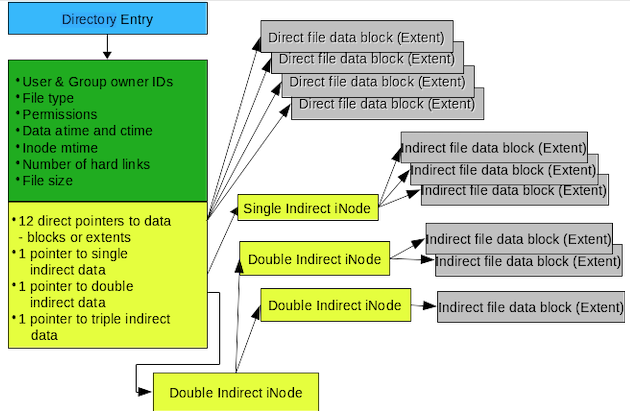
\includegraphics[width=0.8\linewidth,keepaspectratio]{images/inodes.png}
\end{center}

\end{frame}

\section{Распределенные файловые системы}

\begin{frame}
\frametitle{Понятие распределенной файловой системы}

\begin{definitionbox}[DFS]
  Файловая система, которая хранит файлы на нескольких серверах или компьютерах, объединяя их в единое виртуальное пространство имён.
\end{definitionbox}

\textbf{Преимущества:}
\begin{itemize}
  \item \textbf{Масштабируемость} — добавляем новые серверы для увеличения хранилища
  \item \textbf{Отказоустойчивость} — потеря одного сервера не потеряет всё
  \item \textbf{Распределённый доступ} — несколько клиентов работают параллельно
  \item \textbf{Производительность} — балансировка нагрузки между серверами
\end{itemize}

\textbf{Примеры:} NFS, AFS, GFS, HDFS, Ceph, Lustre, IPFS

\end{frame}

% ...

\begin{frame}
\frametitle{Отличия от обычных файловых систем}

\begin{columns}
  \column{0.5\textwidth}
  \textbf{Обычная ФС (локальная):}
  \begin{itemize}
    \item Одна машина
    \item Простая архитектура
    \item Быстрый доступ
    \item Ограничены ёмкостью диска
  \end{itemize}

  \column{0.5\textwidth}
  \textbf{Распределённая ФС:}
  \begin{itemize}
    \item Несколько машин
    \item Сложная архитектура
    \item Задержки сети
    \item Масштабируются горизонтально
  \end{itemize}
\end{columns}

\vspace{0.3cm}

\textbf{Дополнительные вызовы DFS:}
\begin{itemize}
  \item \textbf{Консистентность} — синхронизация данных между узлами
  \item \textbf{Отказы} — потеря связи, сбой сервера
  \item \textbf{Производительность} — задержки сети усложняют оптимизацию
  \item \textbf{Безопасность} — защита передачи данных по сети
\end{itemize}

\end{frame}

\begin{frame}
\frametitle{Типы распределённых файловых систем}

\begin{enumerate}
  \item \textbf{Централизованные DFS}
  \begin{itemize}
    \item Центральный сервер управляет доступом и распределением
    \item Примеры: NFS, AFS
  \end{itemize}

  \vspace{0.2cm}

  \item \textbf{Распределённые (параллельные) DFS}
  \begin{itemize}
    \item Серверы метаданных управляют пространством имён
    \item Серверы хранилища отвечают за данные
    \item Примеры: GFS, HDFS, Lustre, Ceph
  \end{itemize}

  \vspace{0.2cm}

  \item \textbf{P2P DFS}
  \begin{itemize}
    \item Каждый узел одновременно клиент и сервер
    \item Нет центрального управления
    \item Примеры: IPFS, BitTorrent, DHT
  \end{itemize}
\end{enumerate}

\end{frame}

\begin{frame}
\frametitle{Amazon S3: отличия от DFS}

\begin{center}
    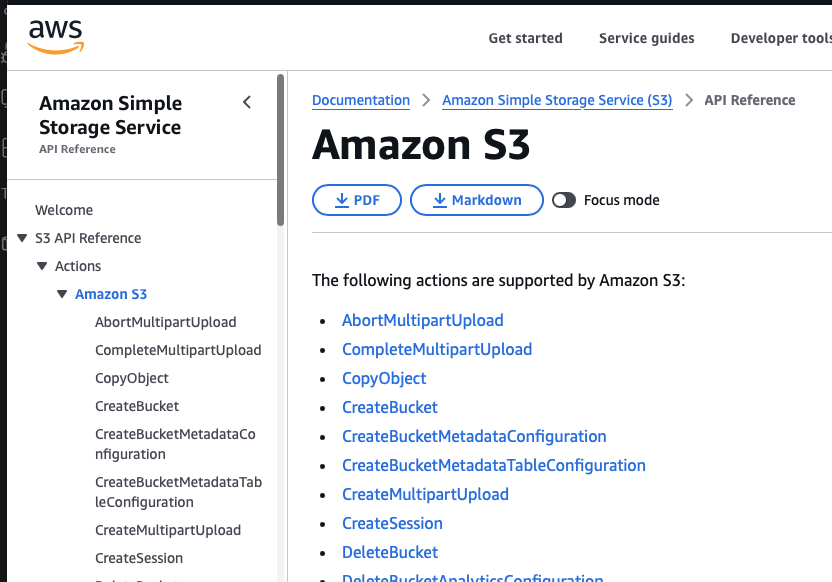
\includegraphics[width=0.8\linewidth,keepaspectratio]{images/s3_api.png}
\end{center}

\href{https://aws.amazon.com/ru/about-aws/global-infrastructure/}{Что такое AWS?}

\end{frame}

\section{Централизованные DFS: NFS, AFS}

\begin{frame}
\frametitle{NFS (Network File System)}

\textbf{История:} разработана Sun Microsystems в 1984 году

\textbf{Основная идея:}
\begin{itemize}
  \item Монтирование удалённой ФС как локальной директории
  \item Клиенты обращаются к серверу через RPC (Remote Procedure Call)
  \item Прозрачный доступ к файлам
\end{itemize}

\textbf{Архитектура:}
\begin{itemize}
  \item \textbf{NFS Server} — хранит файлы, обрабатывает запросы
  \item \textbf{NFS Client} — кэширует данные локально
  \item Протокол: NFSv3 (stateless), NFSv4 (с состоянием)
\end{itemize}

\textbf{Плюсы:} простота, стандарт в UNIX/Linux экосистеме

\textbf{Минусы:} центральный сервер — узкое место, проблемы с отказоустойчивостью

\end{frame}

\begin{frame}
\frametitle{NFS API}

\begin{center}
    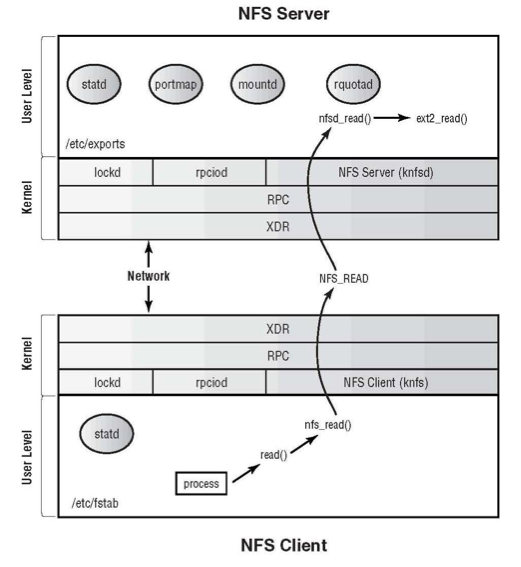
\includegraphics[width=0.5\linewidth,keepaspectratio]{images/nfs_api.png}
\end{center}

\href{https://www.fsl.cs.sunysb.edu/~ezk/cse506-s19/handouts/ch1+6.pdf}{Подробнее}

\end{frame}

\begin{frame}
\frametitle{Сравнение с другими похожими протоколами}

\begin{center}
    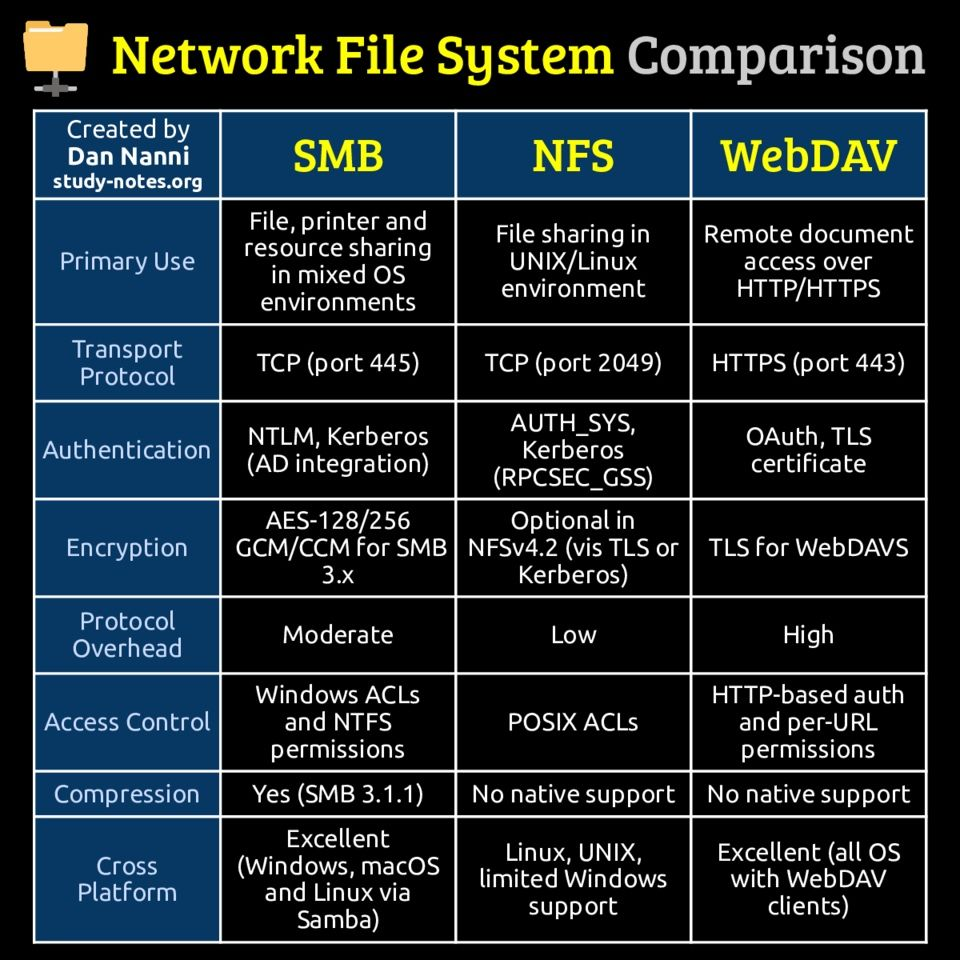
\includegraphics[width=0.65\linewidth,keepaspectratio]{images/nfs_comparison.jpeg}
\end{center}

\end{frame}

\begin{frame}
\frametitle{AFS (Andrew File System)}

\textbf{История:} создана в Carnegie Mellon University (1980-е)

\textbf{Особенности:}
\begin{itemize}
  \item Целое-файловое кэширование на клиентах
  \item Нарушение кэша (cache invalidation) через callbacks
  \item Иерархическое управление (ячейки — cells)
  \item Безопасность встроена (Kerberos)
\end{itemize}

\textbf{Архитектура:}
\begin{itemize}
  \item \textbf{Vice} — серверная часть
  \item \textbf{Venus} — клиентская часть
  \item Данные обмениваются целыми файлами, не блоками
\end{itemize}

\textbf{Сравнение с NFS:} AFS лучше для распределённых сетей с высокой задержкой, благодаря кэшированию

\end{frame}

\begin{frame}
\frametitle{AFS: картинка}

\begin{center}
    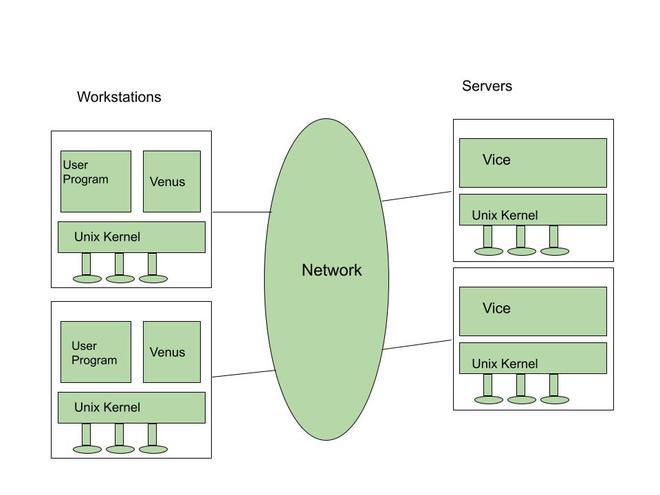
\includegraphics[width=0.9\linewidth,keepaspectratio]{images/afs.jpg}
\end{center}

\end{frame}

\section{Параллельные DFS: GFS, HDFS}

\begin{frame}
\frametitle{GFS (Google File System)}

\textbf{Контекст:} разработана Google для хранения петабайтов данных на тысячах дешёвых серверов

\textbf{Архитектура:}
\begin{itemize}
  \item \textbf{Master} — управляет метаданными (одна копия, реплицирована)
  \item \textbf{Chunkservers} — хранят данные в chunks по 64 MB
  \item \textbf{Clients} — читают и пишут через master и chunkservers
\end{itemize}

\textbf{Особенности:}
\begin{itemize}
  \item Высокая пропускная способность важнее низкой задержки
  \item Append-only семантика (добавления, не перезаписи)
  \item Ленивая репликация chunks
  \item Восстановление после сбоев на лету
\end{itemize}

\textbf{Применение:} MapReduce, поисковые индексы, аналитика

\end{frame}

\begin{frame}
\frametitle{Подробнее}

\href{http://fac-staff.seattleu.edu/zhuy/web/teaching/Spring10/csse550/GFS-lecture.pdf}{Подробнее про GFS}

\end{frame}

\begin{frame}
\frametitle{HDFS (Hadoop Distributed File System)}

\textbf{История:} вдохновлена GFS, open-source реализация для Hadoop проекта

\textbf{Архитектура:}
\begin{itemize}
  \item \textbf{NameNode} — master, управляет неймспейсом
  \item \textbf{DataNodes} — хранят блоки (по умолчанию 128 MB или 256 MB)
  \item \textbf{Secondary NameNode} — помощник для контрольных точек
  \item Репликация блоков (по умолчанию 3 копии)
\end{itemize}

\textbf{Особенности:}
\begin{itemize}
  \item Write-once модель (один раз запись, затем только чтение)
  \item Rack-aware placement (учитывает сетевую топологию)
  \item Heartbeats для мониторинга здоровья узлов
\end{itemize}

\textbf{Применение:} распределённые вычисления (MapReduce, Spark), Big Data аналитика

\end{frame}

\begin{frame}
\frametitle{Что такое Rack Awareness?}

\begin{center}
    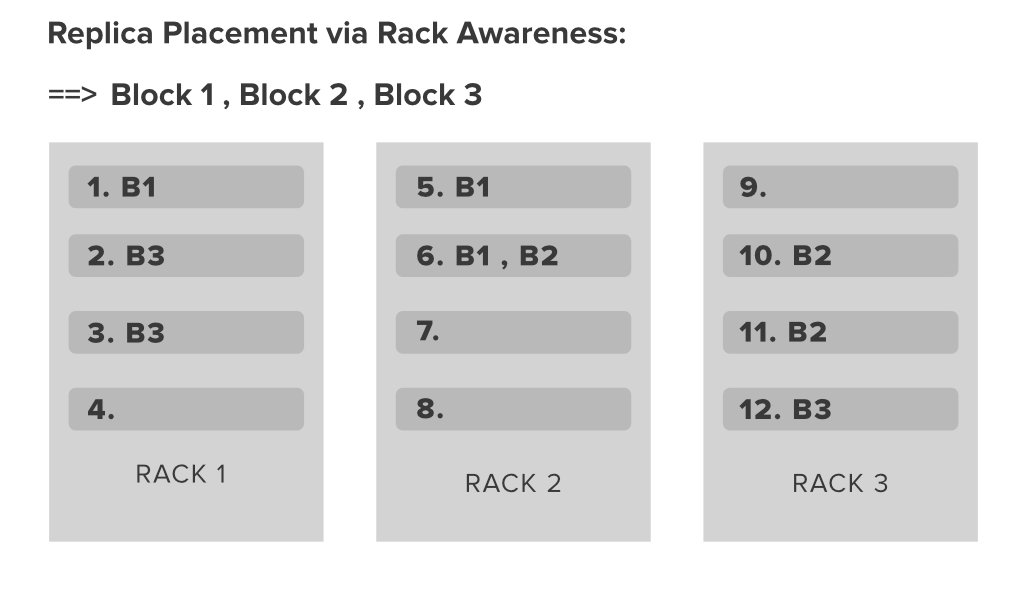
\includegraphics[width=0.9\linewidth,keepaspectratio]{images/hadoop-rack-awareness.png}
\end{center}

Помогает оптимизировать размещение данных и реплик:
чтобы минимизировать сетевой трафик между узлами и повысить отказоустойчивость
(\href{https://www.geeksforgeeks.org/big-data/hadoop-rack-and-rack-awareness/}{подробнее})

\end{frame}

\begin{frame}
\frametitle{Архитектура}

\begin{center}
    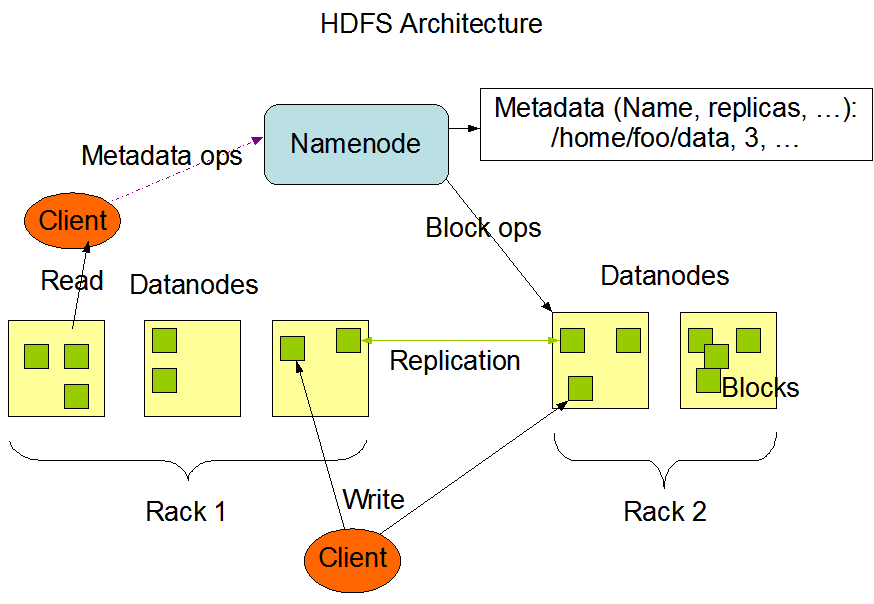
\includegraphics[width=0.85\linewidth,keepaspectratio]{images/hdfsarchitecture.png}
\end{center}

\href{https://hadoop.apache.org/docs/r1.2.1/hdfs_design.html}{подробнее}

\end{frame}

\begin{frame}
\frametitle{Архитектура}

\href{https://cse.buffalo.edu/~epmikida/teaching/sp23/cse487/slides/lec14.pdf}{подробнее 1}

\href{https://www.cs.ucr.edu/~eldawy/21SCS167/slides/CS167-03-HDFS.pdf}{подробнее 2}

\end{frame}

\section{Peer-to-peer DFS: IPFS}

\begin{frame}
\frametitle{IPFS (InterPlanetary File System)}

\textbf{История:} создана Juan Benet (Protocol Labs), опубликована в 2015 году

\textbf{Основная идея:}
\begin{itemize}
  \item Децентрализованная файловая система на основе P2P сети
  \item Адресация по содержимому (content-addressing), а не по локации
  \item Вдохновлена BitTorrent, Git, DHT
\end{itemize}

\textbf{Ключевые концепции:}
\begin{itemize}
  \item \textbf{IPFS hashes} — контентные хэши (SHA-256)
  \item \textbf{Merkle DAG} — направленный ациклический граф (как в Git)
  \item \textbf{DHT} — распределённая таблица хеширования для поиска
  \item \textbf{Кэширование} — промежуточные узлы кэшируют популярные данные
\end{itemize}

% \textbf{Преимущества:}
% \begin{itemize}
%   \item Резильентность — потеря узлов не влияет на сеть
%   \item Полоса пропускания — контент скачивается с ближайших узлов
%   \item Историчность — как Git, сохраняется вся история
% \end{itemize}

\textbf{Применение:} веб-контент, научные данные, медиа-файлы, Web3

\end{frame}

\begin{frame}
\frametitle{IPFS vs традиционный HTTP}

\begin{columns}
  \column{0.5\textwidth}
  \textbf{HTTP:}
  \begin{itemize}
    \item Client-server
    \item Адресация по локации
    \item Зависит от доступности сервера
    \item Единая точка отказа
  \end{itemize}

  \column{0.5\textwidth}
  \textbf{IPFS:}
  \begin{itemize}
    \item P2P
    \item Адресация по контенту
    \item Доступна пока существует копия
    \item Распределённая надежность
  \end{itemize}
\end{columns}

\vspace{0.3cm}

\textbf{Примеры адресов:}

\begin{itemize}
  \item HTTP: \texttt{http://example.com/image.jpg}
  \item IPFS: \texttt{ipfs://QmR35Vz5z...}
\end{itemize}

Хэш однозначно идентифицирует содержимое независимо от расположения.

\end{frame}

\begin{frame}
\frametitle{Merkle Tree}

\begin{center}
    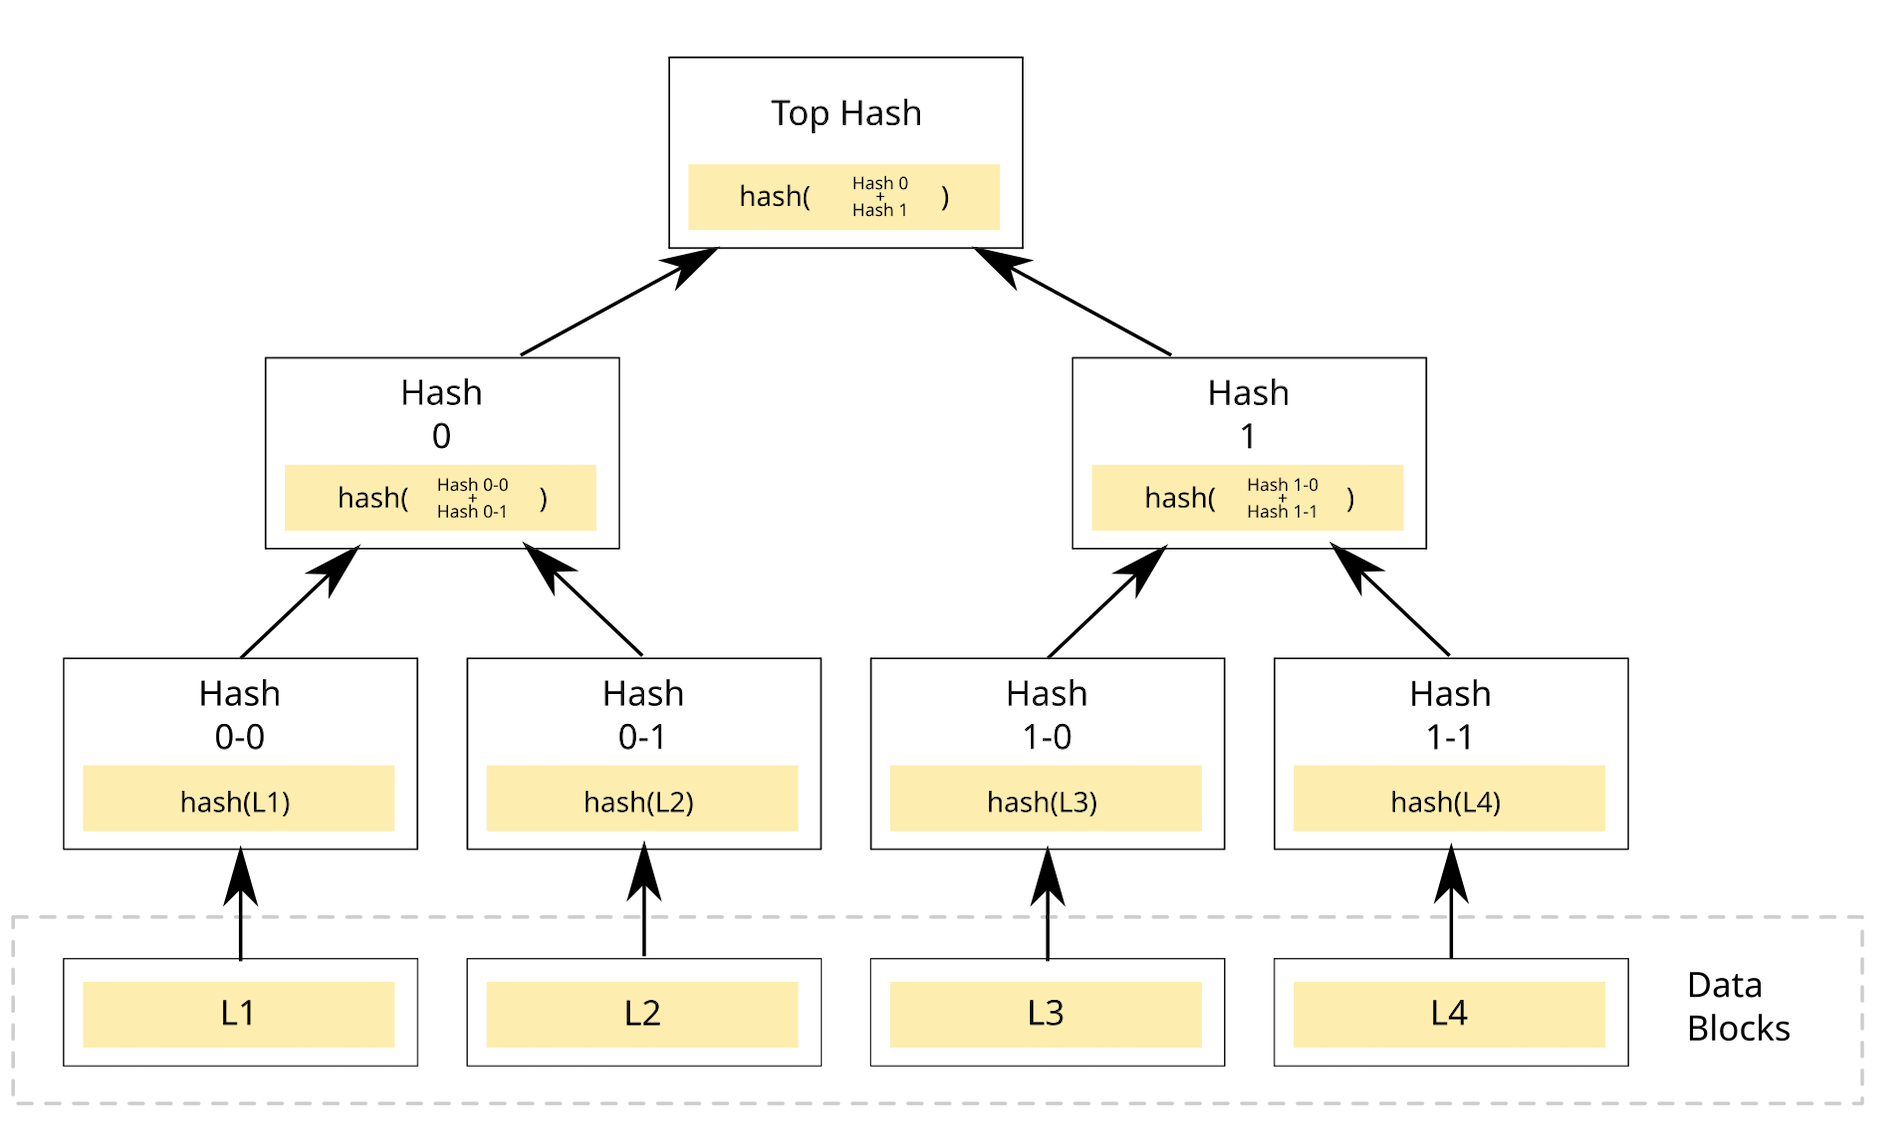
\includegraphics[width=0.85\linewidth,keepaspectratio]{images/merkle_tree.png}
\end{center}

\href{https://docs.ipfs.tech/concepts/lifecycle/\#_1-content-addressing-merkleizing}{подробнее}

\end{frame}

\section{Полезные техники вокруг данных}

\begin{frame}
\frametitle{RAID}

\href{https://ru.wikipedia.org/wiki/RAID}{подробнее}

\end{frame}

\begin{frame}
\frametitle{Erasure coding}

\href{https://ytsaurus.tech/docs/ru/user-guide/storage/replication}{подробнее}

\end{frame}

\begin{frame}
\frametitle{Consistent hashing}

\href{https://www.geeksforgeeks.org/system-design/sharding-vs-consistent-hashing/}{подробнее}

\end{frame}

\begin{frame}
\frametitle{Итоги}

\begin{itemize}
    \item Через неделю дедлайн по домашнему заданию 4 (Raft)
\end{itemize}

\end{frame}

\end{document}